\documentclass{minimal}

\usepackage{pgf,tikz,pgfplots,tkz-euclide}
\usepackage{tikz-3dplot}
\pgfplotsset{compat=1.15}
\usepackage{mathrsfs}
\usepackage{amsmath}
\allowdisplaybreaks[4]
\usetikzlibrary{arrows,arrows.meta,angles,quotes,automata,math}
\usetikzlibrary{calc,fadings,decorations.pathreplacing}
\usetikzlibrary{shadings,intersections}
\usetikzlibrary{3d}
%\usepackage{amsthm}
\usepackage{wrapfig}
\usepackage{gensymb}
\usepackage{subfigure} 
\usepackage{physics}
\usepackage{diagbox}

\begin{document}
\begingroup

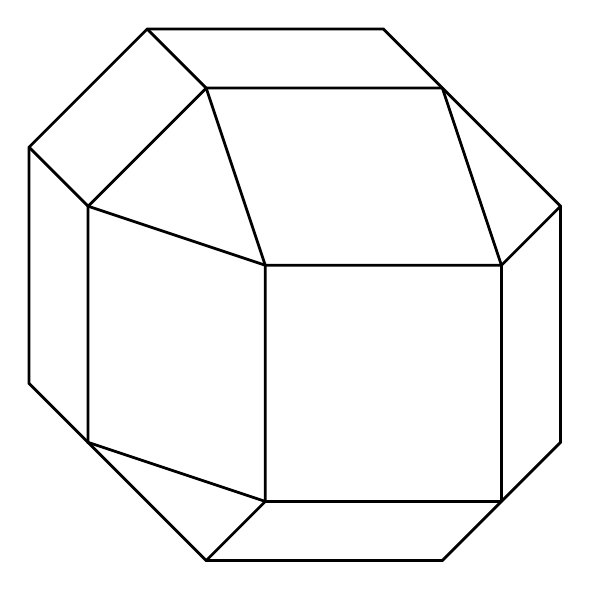
\begin{tikzpicture}[scale=1.5]
\coordinate[] (A) at (0,0);
\coordinate[] (S) at (1, -1);
\coordinate[] (T) at (0.5, 0.5);
\coordinate[] (U) at (-0.5, -0.5);
\coordinate[] (A1) at (-2, 1);
\coordinate[] (E1) at (1, -4);
\coordinate[] (F1) at (-0.5, -3.5);
\coordinate[] (I1) at (1, -3);
\coordinate[] (J1) at (-0.5, -2.5);
\coordinate[] (L1) at (3, -3);
\coordinate[] (M1) at (3, -1);
\coordinate[] (N1) at (2.5, 0.5);
\coordinate[] (O1) at (-1, 0);
\coordinate[] (P1) at (-1, -2);
\coordinate[] (Q1) at (0, 1);
\coordinate[] (R1) at (2, 1);
\coordinate[] (B) at (0.5,-3.5);
\coordinate[] (C) at (2.5,-3.5);
\coordinate[] (D) at (3.5,-0.5);
\coordinate[] (E) at (3.5, -2.5);


\draw [line width=1pt] (O1) -- (P1) -- (J1) -- (B) -- (C) -- (L1) -- (E) -- (D) -- (N1) -- (R1) -- (Q1) -- cycle;
\draw [line width=1pt] (N1) -- (T) -- (U) -- (J1) -- (I1) -- (L1);
\draw [line width=1pt] (Q1) -- (T) -- (S) -- (I1) -- (B);
\draw [line width=1pt] (O1) -- (U) -- (S) -- (M1) -- (D);
\draw [line width=1pt] (N1) -- (M1) -- (L1);

\end{tikzpicture}
\endgroup
\end{document}
